\documentclass[11pt]{beamer}
\usepackage[T2A]{fontenc}
\usepackage[utf8]{inputenc}
\usepackage[english,russian]{babel}
\usepackage{amssymb,amsfonts,amsmath,mathtext, mathtools}
\usepackage{cite,enumerate,float,indentfirst}
\usepackage{subcaption}

\graphicspath{{images/}}

\usetheme[usetitleprogressbar, usetotalslideindicator, nooffset]{m}

% title page template
\makeatletter
\setbeamertemplate{title page}
{
    \ifx\insertinstitute\@empty\else
    % \insertinstitute is nonempty
    \vspace*{0.5cm}
    \begin{minipage}[b][\paperheight]{\textwidth}
    \begin{minipage}[c]{\textwidth}
      {{
        \begin{center}
        \usebeamerfont{institute}%
        \usebeamercolor[fg]{institute}%
        \insertinstitute%
        \end{center}
      }}
    \end{minipage}
    \fi

    \vspace*{1cm}

    \ifx\inserttitlegraphic\@empty\else
    {% \inserttitlegraphic is nonempty
      \vbox to 0pt
      {% display title graphic without changing the position of other elements
        \vspace*{2em}
        \usebeamercolor[fg]{titlegraphic}%
        \inserttitlegraphic%
      }%
      \nointerlineskip%
    }
    \fi

    \vfill%

  \ifx\inserttitle\@empty\else
    {{% \inserttitle is nonempty
      \raggedright%
      \linespread{1.0}%
      \usebeamerfont{title}%
      \usebeamercolor[fg]{title}%
      \begin{center}
      \scshape \inserttitle%
      \end{center}
    }}
    \fi

    \ifx\insertsubtitle\@empty\else
    {{% \insertsubtitle is nonempty
      \usebeamerfont{subtitle}%
      \usebeamercolor[fg]{subtitle}%
      \centering
      \insertsubtitle%
      \vspace*{0.5em}%
    }}
    \fi

    \begin{tikzpicture}
      \usebeamercolor{title separator}
      \draw[fg] (0, 0) -- (\textwidth, 0);
    \end{tikzpicture}%
    % \vspace*{1em}%

    \ifx\beamer@shortauthor\@empty\else
    {{% \insertauthor is always nonempty by beamer's definition, so we must
      % test another macro which is initialized by \author{...}
      % For details, see http://tex.stackexchange.com/questions/241306/
      \usebeamerfont{author}%
      \usebeamercolor[fg]{author}%
      \insertauthor%
      \par%
      \vspace*{0.25em}
    }}
    \fi

    \ifx\insertdate\@empty\else
    {{% \insertdate is nonempty
      \usebeamerfont{date}%
      \usebeamercolor[fg]{date}%
      \begin{center}
      \insertdate%
      \end{center}
      \par%
    }}
    \fi

    \vfill
    \vspace*{1cm}

  \end{minipage}
}
\makeatother

%%% Переопределение именований %%%

\newcommand{\tr}{\mathrm{Tr}}
\newcommand{\e}{\mathrm{e}}
\renewcommand{\imath}{\mathrm{i}}

\newcommand{\N}{\mathbb{N}}
\newcommand{\Z}{\mathbb{Z}}
\newcommand{\R}{\mathbb{R}}
\newcommand{\exR}{\overline{\mathbb{R}}}
\renewcommand{\P}{\mathbb{P}}
\renewcommand{\C}{\mathbb{C}}

\newcommand{\J}{\mathcal{J}}

\renewcommand{\leq}{\leqslant}
\renewcommand{\geq}{\geqslant}

\renewcommand{\Re}{\mathop{\mathrm{Re}}\nolimits}
\renewcommand{\Im}{\mathop{\mathrm{Im}}\nolimits}

\renewcommand{\d}{\mathrm{d}}

\newcommand{\dd}[2]{\frac{\d{#1}}{\d{#2}}}
\newcommand{\ddd}[2]{\frac{\d^2{#1}}{\d{#2}^2}}
\newcommand{\pd}[2]{\frac{\partial{#1}}{\partial{#2}}}
\newcommand{\pdd}[2]{\frac{\partial^2{#1}}{\partial{#2}^2}}
\newcommand{\pdp}[3]{\frac{\partial^2{#1}}{\partial{#2}\partial{#3}}}
\newcommand{\pdet}[1]{\det\left({#1}\right)}
\renewcommand{\exp}[1]{\mathrm{e}^{#1}}
\newcommand{\half}[1]{\frac{#1}{2}}

\newcommand{\trans}[1]{{#1}^\mathrm{T}}
\newcommand{\op}[1]{\mathrm{#1}}

\newcommand{\E}{\op{E}}
\newcommand{\D}{\op{D}}
\newcommand{\cov}{\op{cov}}
\newcommand{\Dom}{\op{Dom}}
\newcommand{\Ran}{\op{Ran}}

\newcommand*\Diff{\mathop{}\!\mathbin\bigtriangleup}
\DeclarePairedDelimiter\brts{(}{)}
\DeclarePairedDelimiter\sqts{[}{]}
           % Переопределение именований

\institute{\center\footnotesize{Санкт-Петербургский политехнический университет Петра Великого \\ Институт прикладной математики и механики \\ Кафедра прикладной математики и информатики}}
\title{Изучение связей между оценками \\ параметров моделей случайных процессов с помощью копул \\ {\small Выпускная работа бакалавра}}
% \subtitle
\author{\small{%
Выполнил ст. гр. 43601/2: \hfill ~И. П. Дмитриевский\\%
Руководитель:~доц.,~к.ф.-м.н. \hfill ~А. А. Иванков}\\%
\vfill
}
\date{\small{Санкт-Петербург, 2015}}

\begin{document}
\renewcommand{\inserttotalframenumber}{20}
\maketitle

\begin{frame}
\frametitle{Модель случайного процесса}
\begin{equation}\label{eq:x}
X(t) = Z(t) + Y(t)
\end{equation}
\begin{equation}
Z(t) = \mu + \sigma W(t)
\end{equation}
\begin{equation}
Y(t) = \sum_{j=0}^K P_j \cdot I(t - \tau_j) \cdot e^{-\lambda_c(t - \tau_j)}
\end{equation}
\begin{itemize}
  \item $K$~---~число событий, поступивших до момента $t$;
  \item $\tau_j$~---~время возникновения $j$-ого возмущения;
  \item $I$~---~функция Хевисайда;
  \item $\lambda_c$~---~константа, одинаковая для всех событий;
  \item $P_j \sim Pareto(x_m, \alpha)$;
  \item $\Diff\tau_j \sim Exp(\lambda)$;
\end{itemize}
\begin{equation}
(\mu, \sigma, x_m, \alpha, \lambda, \lambda_c)
\end{equation}
\end{frame}

\begin{frame}
\frametitle{Оценивание параметров модели $X(t)$}
\begin{itemize}
  \item Алгоритм оценивания параметров модели процесса \eqref{eq:x} реализован в [Сидоровская, 2015 г.];
  \item В рамках реализованного подхода наиболее критичный этап --- интервальное оценивание;
  \item Интервальное оценивание --- композиция нескольких алгоритмов, доставляющих границы компакта;
\end{itemize}
\begin{equation}
  IE(X(t), \overline{\xi}) \colon X(t) \to \R^{12}
\end{equation}
\begin{itemize}
  \item $\overline{\xi}$ --- вектор параметров алгоритма.
\end{itemize}
\end{frame}

\begin{frame}
\frametitle{Постановка задачи}
Дано:
\begin{itemize}
  \item Оценки границ компактов (результаты вычислительных экспериментов по интервальному оцениванию [Сидоровская, 2015 г.]);
  \item Объём входных данных $\approx 10^6$;
\end{itemize}

Требуется:
\begin{itemize}
  \item Оценить стохастические связи между результатами алгоритма интервального оценивания;
\end{itemize}
\end{frame}

\begin{frame}
\frametitle{Выбранный метод}
\begin{itemize}
  \item Коэффициенты корреляции дают слабое представление о структуре связи;
  \item Более полное изучение связей требует построения оценок совместных распределений;
  \item Копулы --- инструмент для аппроксимации совместных распределений;
\end{itemize}
\end{frame}

\begin{frame}
\begin{center}
\frametitle{Копулы}
Теорема Склара:
\begin{equation}
H(x, y) = C(F(x), G(y))
\end{equation}
\begin{itemize}
  \item Теория копул активно развивается;
  \item Копулы успешно применяются для решения различных прикладных задач;
  \item Копулы являются гибким инструментом для исследования стохастических связей;
\end{itemize}
\end{center}
\end{frame}

\begin{frame}
\begin{center}
\frametitle{Аппроксимируемые распределения}
\begin{itemize}
  \item Пусть $s$ --- модельное значение параметра $\sigma$, для которого получены $\sigma_1, \sigma_2$ --- оценки границ компакта;
  \item Определим случайную величину $\omega_{(\sigma = s)}$:
  \begin{itemize}
    \item $\omega_{(\sigma = s)}(s \notin [\sigma_1, \sigma_2]) = 0$;
    \item $\omega_{(\sigma = s)}(s \in [\sigma_1, \sigma_2]) = 1$;
  \end{itemize}
  \item Построим аппроксимацию распределения $\widehat{p}_{(\sigma = s)} = \P\{\, \omega_{(\sigma = s)} = 1\,\}$;
  \item Аналогичные построения выполняются для всех пар параметров;
\end{itemize}
\end{center}
\end{frame}

\begin{frame}
\begin{center}
\frametitle{Созданный и использовавшийся инструментарий}
\begin{itemize}
  \item Созданный программный пакет на я. п. \texttt{C++} позволяет:
    \begin{itemize}
      \item строить вероятностные модели в форме композиции распределений и копул;
      \item строить эмпирические аппроксимации копул;
      \item экспортировать результаты аппроксимации в формате, совместимом с \texttt{gnuplot};
    \end{itemize}
  \item \texttt{gnuplot} --- утилита c богатым выбором выходных форматов, позволяющая визуализировать данные;
\end{itemize}
\end{center}
\end{frame}

\begin{frame}
\frametitle{Метод отражений}
\begin{equation}
  ({U}_i, {V}) = (F_X(X), F_Y(Y));
\end{equation}
\begin{itemize}
  \item Алгоритм аппроксимации использует $(\widehat{U}_i, \widehat{V}_i) = (F_{X, T}(X_i), F_{Y, T}(Y_i))$;
  \item Дополнительно используются отражения относительно границ и углов области определения копулы (единичного квадрата);
  \item Строится аппроксимация распределения и сглаживается фильтром Гаусса;
\end{itemize}
\end{frame}

\begin{frame}
\begin{center}
\frametitle{Результат аппроксимации методом отражений}
\begin{figure}[H]
  \centering
  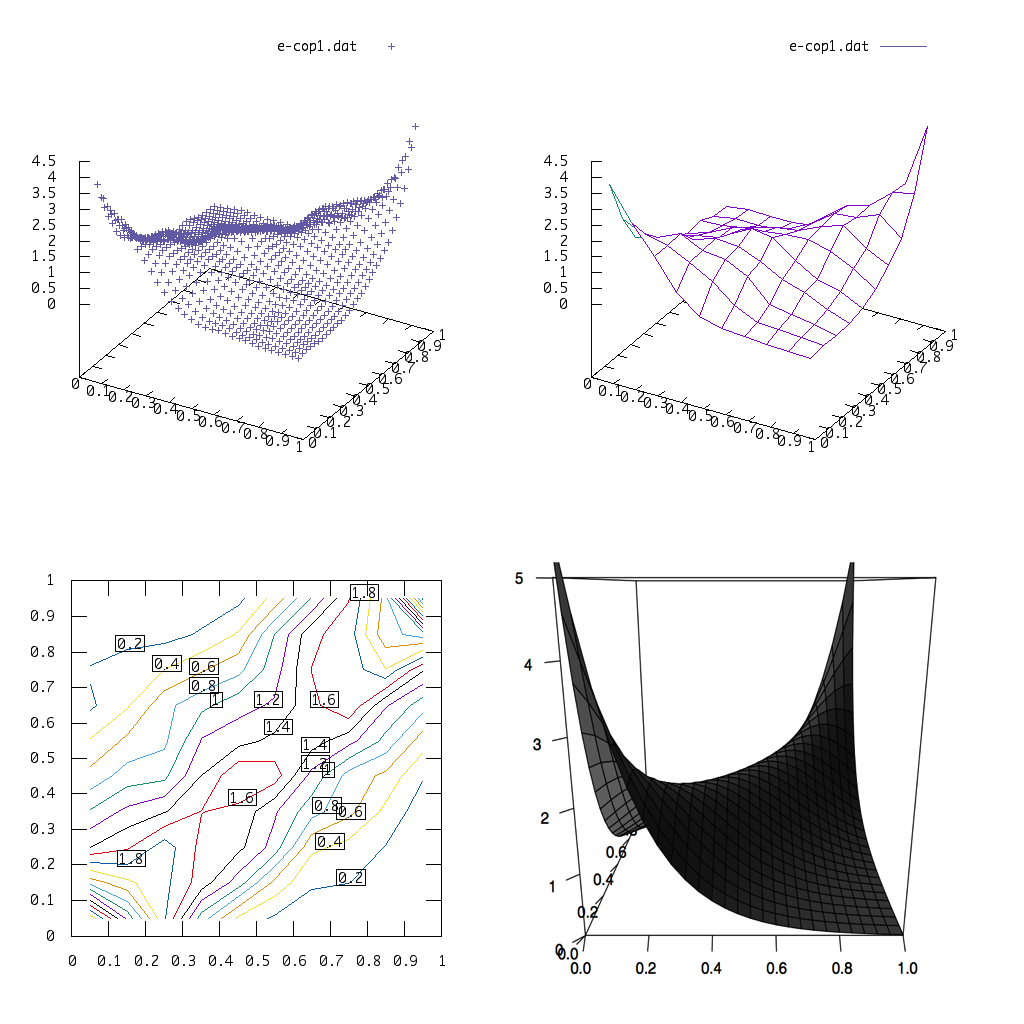
\includegraphics[width=.56\textwidth]{FrankMirror.png}
  \caption{Графики оценённой (метод отражений, 1000 наблюдений) и теоретической плотностей копулы Фрэнка}
\end{figure}
\end{center}
\end{frame}

\begin{frame}
\frametitle{Метод преобразований}
\begin{itemize}
  \item $G$ --- непрерывная функция распределения на $\R$;
  \item $g$ --- положительная плотность $G$;
  \item Плотность $(\widetilde{X}, \widetilde{Y})$, где $\widetilde{X} = G^{-1}(U)$ и $\widetilde{V} = G^{-1}(V)$, равна
\begin{equation}\label{eq:transform_method}
f(x, y) = g(x)g(y)c(G(x), G(y)),
\end{equation}
где $c$ --- аппроксимируемая копула;
\item $f$ аппроксимируется по формуле
\begin{equation}
\widehat{f}(x, y) = \frac{1}{T h^2} \sum_{i=1}^T K\brts*{\frac{x - \widetilde{X}}{h}, \frac{y - \widetilde{Y}}{h}},
\end{equation}
где $K$ --- сглаживающий фильтр.
\end{itemize}
\end{frame}

\begin{frame}
\begin{center}
\frametitle{Результат аппроксимации методом преобразований}
\begin{figure}[H]
  \centering
  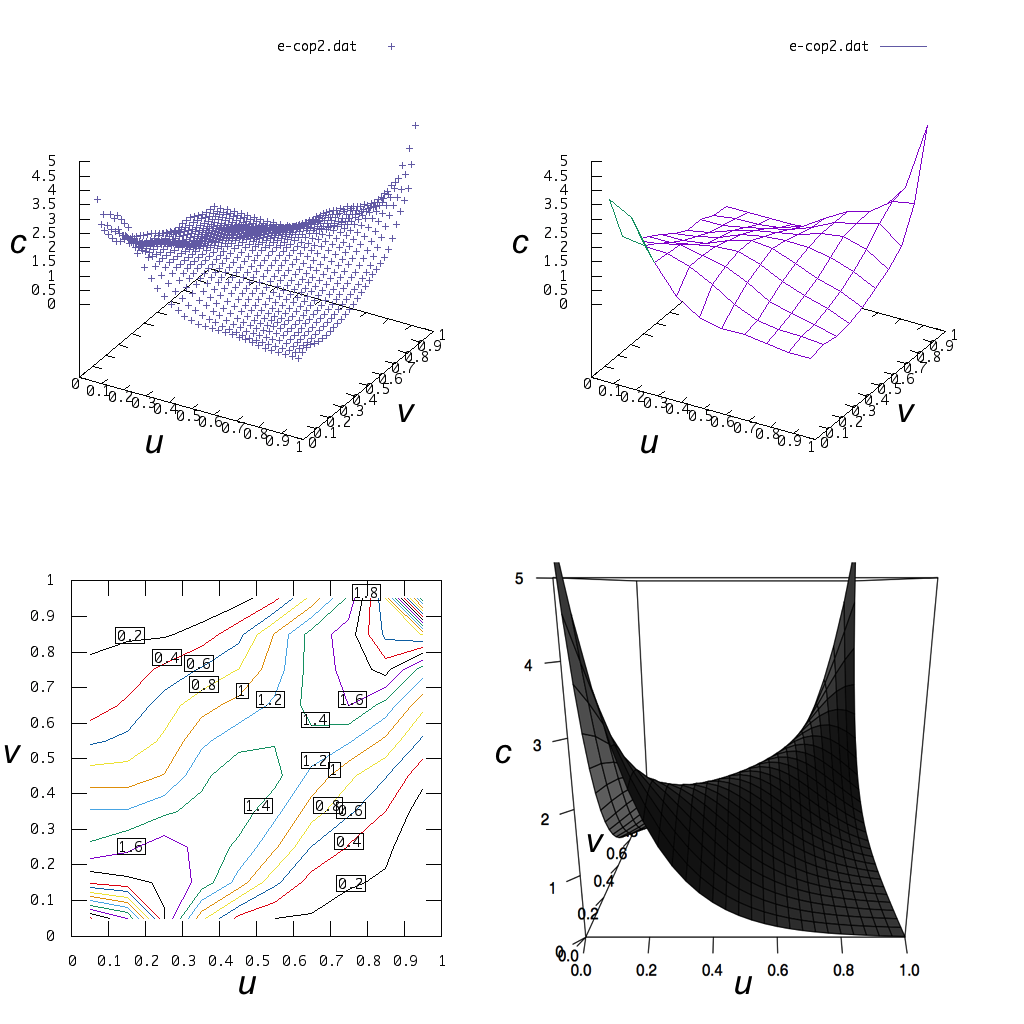
\includegraphics[width=.56\textwidth]{FrankTransform.png}
  \caption{Графики оценённой (метод преобразований, 1000 наблюдений) и теоретической плотностей копулы Фрэнка}
\end{figure}
\end{center}
\end{frame}

\setbeamertemplate{frametitle}
{
  \nointerlineskip
  \begin{beamercolorbox}[wd=\paperwidth,leftskip=0.3cm,rightskip=0.3cm,ht=5.5ex,dp=1.5ex]{frametitle}
    \usebeamerfont{frametitle}%
    \scshape \protect\insertframetitle%
  \end{beamercolorbox}%

  \if@useTitleProgressBar
    \nointerlineskip
    \begin{beamercolorbox}[wd=\paperwidth,ht=0.4pt,dp=0pt]{frametitle}
      \progressbar{\paperwidth}
    \end{beamercolorbox}
  \fi
}
\makeatother

\begin{frame}
\begin{center}
\frametitle{Пример визуализации копулы для оценок границ компактов параметров $\sigma$ и $x_m$}
\resizebox{\columnwidth}{!}{% GNUPLOT: LaTeX picture with Postscript
\begingroup
  \makeatletter
  \providecommand\color[2][]{%
    \GenericError{(gnuplot) \space\space\space\@spaces}{%
      Package color not loaded in conjunction with
      terminal option `colourtext'%
    }{See the gnuplot documentation for explanation.%
    }{Either use 'blacktext' in gnuplot or load the package
      color.sty in LaTeX.}%
    \renewcommand\color[2][]{}%
  }%
  \providecommand\includegraphics[2][]{%
    \GenericError{(gnuplot) \space\space\space\@spaces}{%
      Package graphicx or graphics not loaded%
    }{See the gnuplot documentation for explanation.%
    }{The gnuplot epslatex terminal needs graphicx.sty or graphics.sty.}%
    \renewcommand\includegraphics[2][]{}%
  }%
  \providecommand\rotatebox[2]{#2}%
  \@ifundefined{ifGPcolor}{%
    \newif\ifGPcolor
    \GPcolortrue
  }{}%
  \@ifundefined{ifGPblacktext}{%
    \newif\ifGPblacktext
    \GPblacktextfalse
  }{}%
  % define a \g@addto@macro without @ in the name:
  \let\gplgaddtomacro\g@addto@macro
  % define empty templates for all commands taking text:
  \gdef\gplbacktext{}%
  \gdef\gplfronttext{}%
  \makeatother
  \ifGPblacktext
    % no textcolor at all
    \def\colorrgb#1{}%
    \def\colorgray#1{}%
  \else
    % gray or color?
    \ifGPcolor
      \def\colorrgb#1{\color[rgb]{#1}}%
      \def\colorgray#1{\color[gray]{#1}}%
      \expandafter\def\csname LTw\endcsname{\color{white}}%
      \expandafter\def\csname LTb\endcsname{\color{black}}%
      \expandafter\def\csname LTa\endcsname{\color{black}}%
      \expandafter\def\csname LT0\endcsname{\color[rgb]{1,0,0}}%
      \expandafter\def\csname LT1\endcsname{\color[rgb]{0,1,0}}%
      \expandafter\def\csname LT2\endcsname{\color[rgb]{0,0,1}}%
      \expandafter\def\csname LT3\endcsname{\color[rgb]{1,0,1}}%
      \expandafter\def\csname LT4\endcsname{\color[rgb]{0,1,1}}%
      \expandafter\def\csname LT5\endcsname{\color[rgb]{1,1,0}}%
      \expandafter\def\csname LT6\endcsname{\color[rgb]{0,0,0}}%
      \expandafter\def\csname LT7\endcsname{\color[rgb]{1,0.3,0}}%
      \expandafter\def\csname LT8\endcsname{\color[rgb]{0.5,0.5,0.5}}%
    \else
      % gray
      \def\colorrgb#1{\color{black}}%
      \def\colorgray#1{\color[gray]{#1}}%
      \expandafter\def\csname LTw\endcsname{\color{white}}%
      \expandafter\def\csname LTb\endcsname{\color{black}}%
      \expandafter\def\csname LTa\endcsname{\color{black}}%
      \expandafter\def\csname LT0\endcsname{\color{black}}%
      \expandafter\def\csname LT1\endcsname{\color{black}}%
      \expandafter\def\csname LT2\endcsname{\color{black}}%
      \expandafter\def\csname LT3\endcsname{\color{black}}%
      \expandafter\def\csname LT4\endcsname{\color{black}}%
      \expandafter\def\csname LT5\endcsname{\color{black}}%
      \expandafter\def\csname LT6\endcsname{\color{black}}%
      \expandafter\def\csname LT7\endcsname{\color{black}}%
      \expandafter\def\csname LT8\endcsname{\color{black}}%
    \fi
  \fi
    \setlength{\unitlength}{0.0500bp}%
    \ifx\gptboxheight\undefined%
      \newlength{\gptboxheight}%
      \newlength{\gptboxwidth}%
      \newsavebox{\gptboxtext}%
    \fi%
    \setlength{\fboxrule}{0.5pt}%
    \setlength{\fboxsep}{1pt}%
\begin{picture}(9070.00,4534.00)%
    \gplgaddtomacro\gplbacktext{%
    }%
    \gplgaddtomacro\gplfronttext{%
      \csname LTb\endcsname%
      \put(2863,4030){\makebox(0,0)[r]{\strut{}$\widehat{p}_\sigma=2.12132$, $\widehat{p}_\lambda=15$}}%
      \csname LTb\endcsname%
      \put(683,1188){\makebox(0,0){\strut{}\ft $0$}}%
      \put(1067,1084){\makebox(0,0){\strut{}\ft $0.2$}}%
      \put(1451,979){\makebox(0,0){\strut{}\ft $0.4$}}%
      \put(1835,875){\makebox(0,0){\strut{}\ft $0.6$}}%
      \put(2219,771){\makebox(0,0){\strut{}\ft $0.8$}}%
      \put(2602,667){\makebox(0,0){\strut{}\ft $1$}}%
      \put(1436,797){\makebox(0,0){\strut{}$\widehat{p}_\sigma$}}%
      \put(2787,710){\makebox(0,0){\strut{}\ft $0$}}%
      \put(3008,891){\makebox(0,0){\strut{}\ft $0.2$}}%
      \put(3230,1071){\makebox(0,0){\strut{}\ft $0.4$}}%
      \put(3452,1252){\makebox(0,0){\strut{}\ft $0.6$}}%
      \put(3673,1433){\makebox(0,0){\strut{}\ft $0.8$}}%
      \put(3895,1613){\makebox(0,0){\strut{}\ft $1$}}%
      \put(3706,1083){\makebox(0,0){\strut{}$\widehat{p}_\lambda$}}%
      \put(627,1886){\makebox(0,0)[r]{\strut{}\ft $0$}}%
      \put(627,2168){\makebox(0,0)[r]{\strut{}\ft $3$}}%
      \put(627,2450){\makebox(0,0)[r]{\strut{}\ft $6$}}%
      \put(627,2733){\makebox(0,0)[r]{\strut{}\ft $9$}}%
      \put(627,3016){\makebox(0,0)[r]{\strut{}\ft $12$}}%
      \put(-171,2487){\makebox(0,0){\strut{}$\widehat{c}$}}%
    }%
    \gplgaddtomacro\gplbacktext{%
    }%
    \gplgaddtomacro\gplfronttext{%
      \csname LTb\endcsname%
      \put(5223,578){\makebox(0,0){\strut{}\ft $0$}}%
      \put(5855,578){\makebox(0,0){\strut{}\ft $0.2$}}%
      \put(6487,578){\makebox(0,0){\strut{}\ft $0.4$}}%
      \put(7117,578){\makebox(0,0){\strut{}\ft $0.6$}}%
      \put(7749,578){\makebox(0,0){\strut{}\ft $0.8$}}%
      \put(8381,578){\makebox(0,0){\strut{}\ft $1$}}%
      \put(6802,248){\makebox(0,0){\strut{}$\widehat{p}_\sigma$}}%
      \put(5035,891){\makebox(0,0)[r]{\strut{}\ft $0$}}%
      \put(5035,1486){\makebox(0,0)[r]{\strut{}\ft $0.2$}}%
      \put(5035,2080){\makebox(0,0)[r]{\strut{}\ft $0.4$}}%
      \put(5035,2674){\makebox(0,0)[r]{\strut{}\ft $0.6$}}%
      \put(5035,3268){\makebox(0,0)[r]{\strut{}\ft $0.8$}}%
      \put(5035,3863){\makebox(0,0)[r]{\strut{}\ft $1$}}%
      \put(4309,2377){\rotatebox{-270}{\makebox(0,0){\strut{}$\widehat{p}_\lambda$}}}%
    }%
    \gplbacktext
    \put(0,0){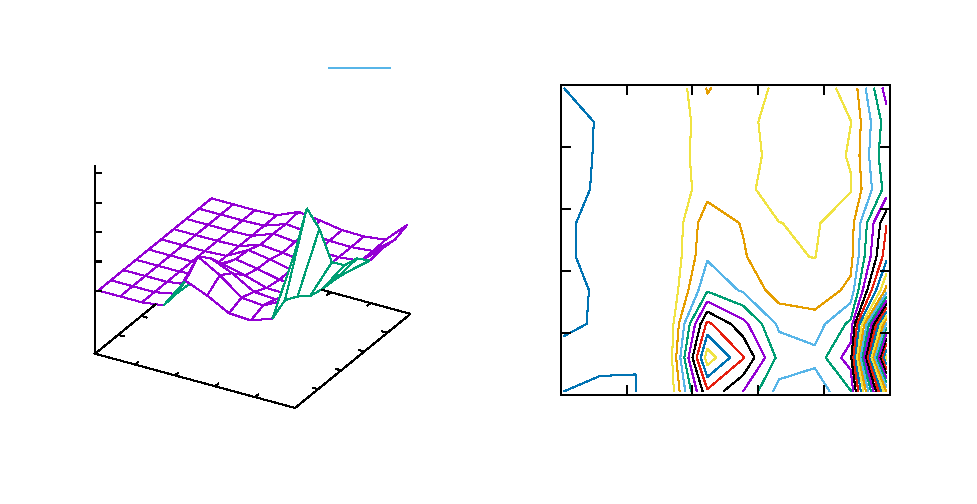
\includegraphics{images/plots/plot_11_40_1000}}%
    \gplfronttext
  \end{picture}%
\endgroup
}
{\small Рис. 3 Плотность распределения указанной копулы}
\end{center}
\end{frame}

\setbeamertemplate{frametitle}
{
  \nointerlineskip
  \begin{beamercolorbox}[wd=\paperwidth,leftskip=0.3cm,rightskip=0.3cm,ht=2.5ex,dp=1.5ex]{frametitle}
    \usebeamerfont{frametitle}%
    \scshape \protect\insertframetitle%
  \end{beamercolorbox}%

  \if@useTitleProgressBar
    \nointerlineskip
    \begin{beamercolorbox}[wd=\paperwidth,ht=0.4pt,dp=0pt]{frametitle}
      \progressbar{\paperwidth}
    \end{beamercolorbox}
  \fi
}
\makeatother

\begin{frame}
\begin{center}
\frametitle{График плотности распределения ординат $Z(t)$ и $Y(t)$}
{\small Рис. 4 Плотности распределения ординат указанных процессов при фиксированном $t$}
\resizebox{\columnwidth}{!}{% GNUPLOT: LaTeX picture with Postscript
\begingroup
  \makeatletter
  \providecommand\color[2][]{%
    \GenericError{(gnuplot) \space\space\space\@spaces}{%
      Package color not loaded in conjunction with
      terminal option `colourtext'%
    }{See the gnuplot documentation for explanation.%
    }{Either use 'blacktext' in gnuplot or load the package
      color.sty in LaTeX.}%
    \renewcommand\color[2][]{}%
  }%
  \providecommand\includegraphics[2][]{%
    \GenericError{(gnuplot) \space\space\space\@spaces}{%
      Package graphicx or graphics not loaded%
    }{See the gnuplot documentation for explanation.%
    }{The gnuplot epslatex terminal needs graphicx.sty or graphics.sty.}%
    \renewcommand\includegraphics[2][]{}%
  }%
  \providecommand\rotatebox[2]{#2}%
  \@ifundefined{ifGPcolor}{%
    \newif\ifGPcolor
    \GPcolortrue
  }{}%
  \@ifundefined{ifGPblacktext}{%
    \newif\ifGPblacktext
    \GPblacktextfalse
  }{}%
  % define a \g@addto@macro without @ in the name:
  \let\gplgaddtomacro\g@addto@macro
  % define empty templates for all commands taking text:
  \gdef\gplbacktext{}%
  \gdef\gplfronttext{}%
  \makeatother
  \ifGPblacktext
    % no textcolor at all
    \def\colorrgb#1{}%
    \def\colorgray#1{}%
  \else
    % gray or color?
    \ifGPcolor
      \def\colorrgb#1{\color[rgb]{#1}}%
      \def\colorgray#1{\color[gray]{#1}}%
      \expandafter\def\csname LTw\endcsname{\color{white}}%
      \expandafter\def\csname LTb\endcsname{\color{black}}%
      \expandafter\def\csname LTa\endcsname{\color{black}}%
      \expandafter\def\csname LT0\endcsname{\color[rgb]{1,0,0}}%
      \expandafter\def\csname LT1\endcsname{\color[rgb]{0,1,0}}%
      \expandafter\def\csname LT2\endcsname{\color[rgb]{0,0,1}}%
      \expandafter\def\csname LT3\endcsname{\color[rgb]{1,0,1}}%
      \expandafter\def\csname LT4\endcsname{\color[rgb]{0,1,1}}%
      \expandafter\def\csname LT5\endcsname{\color[rgb]{1,1,0}}%
      \expandafter\def\csname LT6\endcsname{\color[rgb]{0,0,0}}%
      \expandafter\def\csname LT7\endcsname{\color[rgb]{1,0.3,0}}%
      \expandafter\def\csname LT8\endcsname{\color[rgb]{0.5,0.5,0.5}}%
    \else
      % gray
      \def\colorrgb#1{\color{black}}%
      \def\colorgray#1{\color[gray]{#1}}%
      \expandafter\def\csname LTw\endcsname{\color{white}}%
      \expandafter\def\csname LTb\endcsname{\color{black}}%
      \expandafter\def\csname LTa\endcsname{\color{black}}%
      \expandafter\def\csname LT0\endcsname{\color{black}}%
      \expandafter\def\csname LT1\endcsname{\color{black}}%
      \expandafter\def\csname LT2\endcsname{\color{black}}%
      \expandafter\def\csname LT3\endcsname{\color{black}}%
      \expandafter\def\csname LT4\endcsname{\color{black}}%
      \expandafter\def\csname LT5\endcsname{\color{black}}%
      \expandafter\def\csname LT6\endcsname{\color{black}}%
      \expandafter\def\csname LT7\endcsname{\color{black}}%
      \expandafter\def\csname LT8\endcsname{\color{black}}%
    \fi
  \fi
    \setlength{\unitlength}{0.0500bp}%
    \ifx\gptboxheight\undefined%
      \newlength{\gptboxheight}%
      \newlength{\gptboxwidth}%
      \newsavebox{\gptboxtext}%
    \fi%
    \setlength{\fboxrule}{0.5pt}%
    \setlength{\fboxsep}{1pt}%
\begin{picture}(4534.00,5668.00)%
    \gplgaddtomacro\gplbacktext{%
      \colorrgb{0.00,0.00,0.00}%
      \put(924,3714){\makebox(0,0)[r]{\strut{}\ft $0$}}%
      \colorrgb{0.00,0.00,0.00}%
      \put(924,3939){\makebox(0,0)[r]{\strut{}\ft $0.2$}}%
      \colorrgb{0.00,0.00,0.00}%
      \put(924,4164){\makebox(0,0)[r]{\strut{}\ft $0.4$}}%
      \colorrgb{0.00,0.00,0.00}%
      \put(924,4390){\makebox(0,0)[r]{\strut{}\ft $0.6$}}%
      \colorrgb{0.00,0.00,0.00}%
      \put(924,4615){\makebox(0,0)[r]{\strut{}\ft $0.8$}}%
      \colorrgb{0.00,0.00,0.00}%
      \put(924,4840){\makebox(0,0)[r]{\strut{}\ft $1$}}%
      \colorrgb{0.00,0.00,0.00}%
      \put(924,5065){\makebox(0,0)[r]{\strut{}\ft $1.2$}}%
      \colorrgb{0.00,0.00,0.00}%
      \put(924,5290){\makebox(0,0)[r]{\strut{}\ft $1.4$}}%
      \colorrgb{0.00,0.00,0.00}%
      \put(1364,3494){\makebox(0,0){\strut{}\ft $-4$}}%
      \colorrgb{0.00,0.00,0.00}%
      \put(1980,3494){\makebox(0,0){\strut{}\ft $-2$}}%
      \colorrgb{0.00,0.00,0.00}%
      \put(2597,3494){\makebox(0,0){\strut{}\ft $0$}}%
      \colorrgb{0.00,0.00,0.00}%
      \put(3213,3494){\makebox(0,0){\strut{}\ft $2$}}%
      \colorrgb{0.00,0.00,0.00}%
      \put(3829,3494){\makebox(0,0){\strut{}\ft $4$}}%
      \colorrgb{0.00,0.00,0.00}%
      \put(2597,3054){\makebox(0,0){\strut{}$Z(t), Y(t)$}}%
      \put(2597,6063){\makebox(0,0){\strut{}}}%
      \put(132,4559){\rotatebox{90}{\makebox(0,0){\strut{}$f(X(t)), f(Y(t))$}}}%
      \put(4401,4559){\rotatebox{90}{\makebox(0,0){\strut{}}}}%
    }%
    \gplgaddtomacro\gplfronttext{%
      \colorrgb{0.00,0.00,0.00}%
      \put(242,4558){\rotatebox{-270}{\makebox(0,0){\strut{}}}}%
      \colorrgb{0.00,0.00,0.00}%
      \put(2596,3208){\makebox(0,0){\strut{}}}%
    }%
    \gplbacktext
    \put(0,0){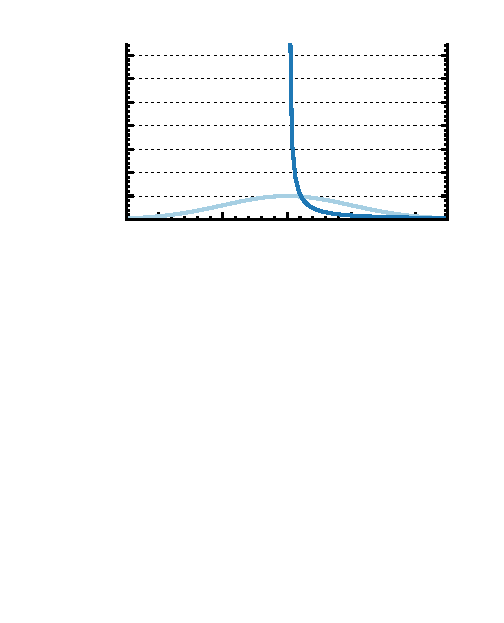
\includegraphics{ZY}}%
    \gplfronttext
  \end{picture}%
\endgroup
}
\end{center}
\end{frame}

\setbeamertemplate{frametitle}
{
  \nointerlineskip
  \begin{beamercolorbox}[wd=\paperwidth,leftskip=0.3cm,rightskip=0.3cm,ht=5.5ex,dp=1.5ex]{frametitle}
    \usebeamerfont{frametitle}%
    \scshape \protect\insertframetitle%
  \end{beamercolorbox}%

  \if@useTitleProgressBar
    \nointerlineskip
    \begin{beamercolorbox}[wd=\paperwidth,ht=0.4pt,dp=0pt]{frametitle}
      \progressbar{\paperwidth}
    \end{beamercolorbox}
  \fi
}
\makeatother

\begin{frame}
\begin{center}
\frametitle{Пример визуализации копулы для оценок границ компактов параметров $\sigma$ и $x_m$ с б\'{о}льшим модельным значением}
\resizebox{\columnwidth}{!}{% GNUPLOT: LaTeX picture with Postscript
\begingroup
  \makeatletter
  \providecommand\color[2][]{%
    \GenericError{(gnuplot) \space\space\space\@spaces}{%
      Package color not loaded in conjunction with
      terminal option `colourtext'%
    }{See the gnuplot documentation for explanation.%
    }{Either use 'blacktext' in gnuplot or load the package
      color.sty in LaTeX.}%
    \renewcommand\color[2][]{}%
  }%
  \providecommand\includegraphics[2][]{%
    \GenericError{(gnuplot) \space\space\space\@spaces}{%
      Package graphicx or graphics not loaded%
    }{See the gnuplot documentation for explanation.%
    }{The gnuplot epslatex terminal needs graphicx.sty or graphics.sty.}%
    \renewcommand\includegraphics[2][]{}%
  }%
  \providecommand\rotatebox[2]{#2}%
  \@ifundefined{ifGPcolor}{%
    \newif\ifGPcolor
    \GPcolortrue
  }{}%
  \@ifundefined{ifGPblacktext}{%
    \newif\ifGPblacktext
    \GPblacktextfalse
  }{}%
  % define a \g@addto@macro without @ in the name:
  \let\gplgaddtomacro\g@addto@macro
  % define empty templates for all commands taking text:
  \gdef\gplbacktext{}%
  \gdef\gplfronttext{}%
  \makeatother
  \ifGPblacktext
    % no textcolor at all
    \def\colorrgb#1{}%
    \def\colorgray#1{}%
  \else
    % gray or color?
    \ifGPcolor
      \def\colorrgb#1{\color[rgb]{#1}}%
      \def\colorgray#1{\color[gray]{#1}}%
      \expandafter\def\csname LTw\endcsname{\color{white}}%
      \expandafter\def\csname LTb\endcsname{\color{black}}%
      \expandafter\def\csname LTa\endcsname{\color{black}}%
      \expandafter\def\csname LT0\endcsname{\color[rgb]{1,0,0}}%
      \expandafter\def\csname LT1\endcsname{\color[rgb]{0,1,0}}%
      \expandafter\def\csname LT2\endcsname{\color[rgb]{0,0,1}}%
      \expandafter\def\csname LT3\endcsname{\color[rgb]{1,0,1}}%
      \expandafter\def\csname LT4\endcsname{\color[rgb]{0,1,1}}%
      \expandafter\def\csname LT5\endcsname{\color[rgb]{1,1,0}}%
      \expandafter\def\csname LT6\endcsname{\color[rgb]{0,0,0}}%
      \expandafter\def\csname LT7\endcsname{\color[rgb]{1,0.3,0}}%
      \expandafter\def\csname LT8\endcsname{\color[rgb]{0.5,0.5,0.5}}%
    \else
      % gray
      \def\colorrgb#1{\color{black}}%
      \def\colorgray#1{\color[gray]{#1}}%
      \expandafter\def\csname LTw\endcsname{\color{white}}%
      \expandafter\def\csname LTb\endcsname{\color{black}}%
      \expandafter\def\csname LTa\endcsname{\color{black}}%
      \expandafter\def\csname LT0\endcsname{\color{black}}%
      \expandafter\def\csname LT1\endcsname{\color{black}}%
      \expandafter\def\csname LT2\endcsname{\color{black}}%
      \expandafter\def\csname LT3\endcsname{\color{black}}%
      \expandafter\def\csname LT4\endcsname{\color{black}}%
      \expandafter\def\csname LT5\endcsname{\color{black}}%
      \expandafter\def\csname LT6\endcsname{\color{black}}%
      \expandafter\def\csname LT7\endcsname{\color{black}}%
      \expandafter\def\csname LT8\endcsname{\color{black}}%
    \fi
  \fi
    \setlength{\unitlength}{0.0500bp}%
    \ifx\gptboxheight\undefined%
      \newlength{\gptboxheight}%
      \newlength{\gptboxwidth}%
      \newsavebox{\gptboxtext}%
    \fi%
    \setlength{\fboxrule}{0.5pt}%
    \setlength{\fboxsep}{1pt}%
\begin{picture}(9070.00,4534.00)%
    \gplgaddtomacro\gplbacktext{%
    }%
    \gplgaddtomacro\gplfronttext{%
      \csname LTb\endcsname%
      \put(2863,4030){\makebox(0,0)[r]{\strut{}$\widehat{p}_\sigma=2.12132$, $\widehat{p}_\lambda=100$}}%
      \csname LTb\endcsname%
      \put(683,1188){\makebox(0,0){\strut{}\ft $0$}}%
      \put(1067,1084){\makebox(0,0){\strut{}\ft $0.2$}}%
      \put(1451,979){\makebox(0,0){\strut{}\ft $0.4$}}%
      \put(1835,875){\makebox(0,0){\strut{}\ft $0.6$}}%
      \put(2219,771){\makebox(0,0){\strut{}\ft $0.8$}}%
      \put(2602,667){\makebox(0,0){\strut{}\ft $1$}}%
      \put(1436,797){\makebox(0,0){\strut{}$\widehat{p}_\sigma$}}%
      \put(2787,710){\makebox(0,0){\strut{}\ft $0$}}%
      \put(3008,891){\makebox(0,0){\strut{}\ft $0.2$}}%
      \put(3230,1071){\makebox(0,0){\strut{}\ft $0.4$}}%
      \put(3452,1252){\makebox(0,0){\strut{}\ft $0.6$}}%
      \put(3673,1433){\makebox(0,0){\strut{}\ft $0.8$}}%
      \put(3895,1613){\makebox(0,0){\strut{}\ft $1$}}%
      \put(3706,1083){\makebox(0,0){\strut{}$\widehat{p}_\lambda$}}%
      \put(627,1885){\makebox(0,0)[r]{\strut{}\ft $0$}}%
      \put(627,2831){\makebox(0,0)[r]{\strut{}\ft $3$}}%
      \put(-171,2487){\makebox(0,0){\strut{}$\widehat{c}$}}%
    }%
    \gplgaddtomacro\gplbacktext{%
    }%
    \gplgaddtomacro\gplfronttext{%
      \csname LTb\endcsname%
      \put(5223,578){\makebox(0,0){\strut{}\ft $0$}}%
      \put(5855,578){\makebox(0,0){\strut{}\ft $0.2$}}%
      \put(6487,578){\makebox(0,0){\strut{}\ft $0.4$}}%
      \put(7117,578){\makebox(0,0){\strut{}\ft $0.6$}}%
      \put(7749,578){\makebox(0,0){\strut{}\ft $0.8$}}%
      \put(8381,578){\makebox(0,0){\strut{}\ft $1$}}%
      \put(6802,248){\makebox(0,0){\strut{}$\widehat{p}_\sigma$}}%
      \put(5035,891){\makebox(0,0)[r]{\strut{}\ft $0$}}%
      \put(5035,1486){\makebox(0,0)[r]{\strut{}\ft $0.2$}}%
      \put(5035,2080){\makebox(0,0)[r]{\strut{}\ft $0.4$}}%
      \put(5035,2674){\makebox(0,0)[r]{\strut{}\ft $0.6$}}%
      \put(5035,3268){\makebox(0,0)[r]{\strut{}\ft $0.8$}}%
      \put(5035,3863){\makebox(0,0)[r]{\strut{}\ft $1$}}%
      \put(4309,2377){\rotatebox{-270}{\makebox(0,0){\strut{}$\widehat{p}_\lambda$}}}%
    }%
    \gplbacktext
    \put(0,0){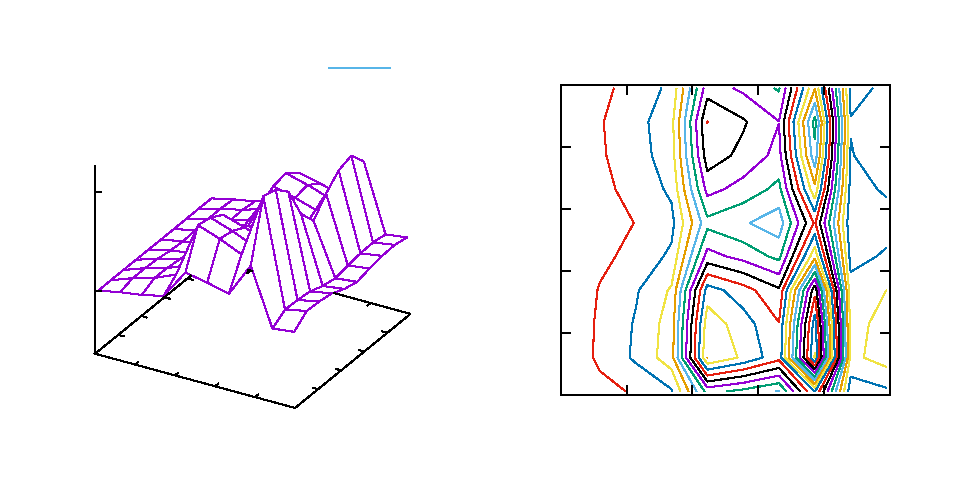
\includegraphics{images/plots/plot_11_41_1000}}%
    \gplfronttext
  \end{picture}%
\endgroup
}
{\small Рис. 5 Плотность распределения указанной копулы}
\end{center}
\end{frame}

\begin{frame}
\begin{center}
\frametitle{Пример визуализации копулы для оценок границ компактов параметров $\sigma$ и $\lambda$}
\resizebox{\columnwidth}{!}{% GNUPLOT: LaTeX picture with Postscript
\begingroup
  \makeatletter
  \providecommand\color[2][]{%
    \GenericError{(gnuplot) \space\space\space\@spaces}{%
      Package color not loaded in conjunction with
      terminal option `colourtext'%
    }{See the gnuplot documentation for explanation.%
    }{Either use 'blacktext' in gnuplot or load the package
      color.sty in LaTeX.}%
    \renewcommand\color[2][]{}%
  }%
  \providecommand\includegraphics[2][]{%
    \GenericError{(gnuplot) \space\space\space\@spaces}{%
      Package graphicx or graphics not loaded%
    }{See the gnuplot documentation for explanation.%
    }{The gnuplot epslatex terminal needs graphicx.sty or graphics.sty.}%
    \renewcommand\includegraphics[2][]{}%
  }%
  \providecommand\rotatebox[2]{#2}%
  \@ifundefined{ifGPcolor}{%
    \newif\ifGPcolor
    \GPcolortrue
  }{}%
  \@ifundefined{ifGPblacktext}{%
    \newif\ifGPblacktext
    \GPblacktextfalse
  }{}%
  % define a \g@addto@macro without @ in the name:
  \let\gplgaddtomacro\g@addto@macro
  % define empty templates for all commands taking text:
  \gdef\gplbacktext{}%
  \gdef\gplfronttext{}%
  \makeatother
  \ifGPblacktext
    % no textcolor at all
    \def\colorrgb#1{}%
    \def\colorgray#1{}%
  \else
    % gray or color?
    \ifGPcolor
      \def\colorrgb#1{\color[rgb]{#1}}%
      \def\colorgray#1{\color[gray]{#1}}%
      \expandafter\def\csname LTw\endcsname{\color{white}}%
      \expandafter\def\csname LTb\endcsname{\color{black}}%
      \expandafter\def\csname LTa\endcsname{\color{black}}%
      \expandafter\def\csname LT0\endcsname{\color[rgb]{1,0,0}}%
      \expandafter\def\csname LT1\endcsname{\color[rgb]{0,1,0}}%
      \expandafter\def\csname LT2\endcsname{\color[rgb]{0,0,1}}%
      \expandafter\def\csname LT3\endcsname{\color[rgb]{1,0,1}}%
      \expandafter\def\csname LT4\endcsname{\color[rgb]{0,1,1}}%
      \expandafter\def\csname LT5\endcsname{\color[rgb]{1,1,0}}%
      \expandafter\def\csname LT6\endcsname{\color[rgb]{0,0,0}}%
      \expandafter\def\csname LT7\endcsname{\color[rgb]{1,0.3,0}}%
      \expandafter\def\csname LT8\endcsname{\color[rgb]{0.5,0.5,0.5}}%
    \else
      % gray
      \def\colorrgb#1{\color{black}}%
      \def\colorgray#1{\color[gray]{#1}}%
      \expandafter\def\csname LTw\endcsname{\color{white}}%
      \expandafter\def\csname LTb\endcsname{\color{black}}%
      \expandafter\def\csname LTa\endcsname{\color{black}}%
      \expandafter\def\csname LT0\endcsname{\color{black}}%
      \expandafter\def\csname LT1\endcsname{\color{black}}%
      \expandafter\def\csname LT2\endcsname{\color{black}}%
      \expandafter\def\csname LT3\endcsname{\color{black}}%
      \expandafter\def\csname LT4\endcsname{\color{black}}%
      \expandafter\def\csname LT5\endcsname{\color{black}}%
      \expandafter\def\csname LT6\endcsname{\color{black}}%
      \expandafter\def\csname LT7\endcsname{\color{black}}%
      \expandafter\def\csname LT8\endcsname{\color{black}}%
    \fi
  \fi
    \setlength{\unitlength}{0.0500bp}%
    \ifx\gptboxheight\undefined%
      \newlength{\gptboxheight}%
      \newlength{\gptboxwidth}%
      \newsavebox{\gptboxtext}%
    \fi%
    \setlength{\fboxrule}{0.5pt}%
    \setlength{\fboxsep}{1pt}%
\begin{picture}(9070.00,4534.00)%
    \gplgaddtomacro\gplbacktext{%
    }%
    \gplgaddtomacro\gplfronttext{%
      \csname LTb\endcsname%
      \put(2863,4030){\makebox(0,0)[r]{\strut{}$\sigma=0.707107$, $x_m=0.01$}}%
      \csname LTb\endcsname%
      \put(683,1188){\makebox(0,0){\strut{}\ft $0$}}%
      \put(1067,1084){\makebox(0,0){\strut{}\ft $0.2$}}%
      \put(1451,979){\makebox(0,0){\strut{}\ft $0.4$}}%
      \put(1835,875){\makebox(0,0){\strut{}\ft $0.6$}}%
      \put(2219,771){\makebox(0,0){\strut{}\ft $0.8$}}%
      \put(2602,667){\makebox(0,0){\strut{}\ft $1$}}%
      \put(1436,797){\makebox(0,0){\strut{}$\widehat{p}_\sigma$}}%
      \put(2787,710){\makebox(0,0){\strut{}\ft $0$}}%
      \put(3008,891){\makebox(0,0){\strut{}\ft $0.2$}}%
      \put(3230,1071){\makebox(0,0){\strut{}\ft $0.4$}}%
      \put(3452,1252){\makebox(0,0){\strut{}\ft $0.6$}}%
      \put(3673,1433){\makebox(0,0){\strut{}\ft $0.8$}}%
      \put(3895,1613){\makebox(0,0){\strut{}\ft $1$}}%
      \put(3706,1083){\makebox(0,0){\strut{}$\widehat{p}_{x_m}$}}%
      \put(627,1886){\makebox(0,0)[r]{\strut{}\ft $0$}}%
      \put(627,2115){\makebox(0,0)[r]{\strut{}\ft $10$}}%
      \put(627,2344){\makebox(0,0)[r]{\strut{}\ft $20$}}%
      \put(627,2572){\makebox(0,0)[r]{\strut{}\ft $30$}}%
      \put(627,2802){\makebox(0,0)[r]{\strut{}\ft $40$}}%
      \put(627,3031){\makebox(0,0)[r]{\strut{}\ft $50$}}%
      \put(-171,2487){\makebox(0,0){\strut{}$\widehat{c}$}}%
    }%
    \gplgaddtomacro\gplbacktext{%
    }%
    \gplgaddtomacro\gplfronttext{%
      \csname LTb\endcsname%
      \put(5223,578){\makebox(0,0){\strut{}\ft $0$}}%
      \put(5855,578){\makebox(0,0){\strut{}\ft $0.2$}}%
      \put(6487,578){\makebox(0,0){\strut{}\ft $0.4$}}%
      \put(7117,578){\makebox(0,0){\strut{}\ft $0.6$}}%
      \put(7749,578){\makebox(0,0){\strut{}\ft $0.8$}}%
      \put(8381,578){\makebox(0,0){\strut{}\ft $1$}}%
      \put(6802,248){\makebox(0,0){\strut{}$\widehat{p}_\sigma$}}%
      \put(5035,891){\makebox(0,0)[r]{\strut{}\ft $0$}}%
      \put(5035,1486){\makebox(0,0)[r]{\strut{}\ft $0.2$}}%
      \put(5035,2080){\makebox(0,0)[r]{\strut{}\ft $0.4$}}%
      \put(5035,2674){\makebox(0,0)[r]{\strut{}\ft $0.6$}}%
      \put(5035,3268){\makebox(0,0)[r]{\strut{}\ft $0.8$}}%
      \put(5035,3863){\makebox(0,0)[r]{\strut{}\ft $1$}}%
      \put(4309,2377){\rotatebox{-270}{\makebox(0,0){\strut{}$\widehat{p}_{x_m}$}}}%
    }%
    \gplbacktext
    \put(0,0){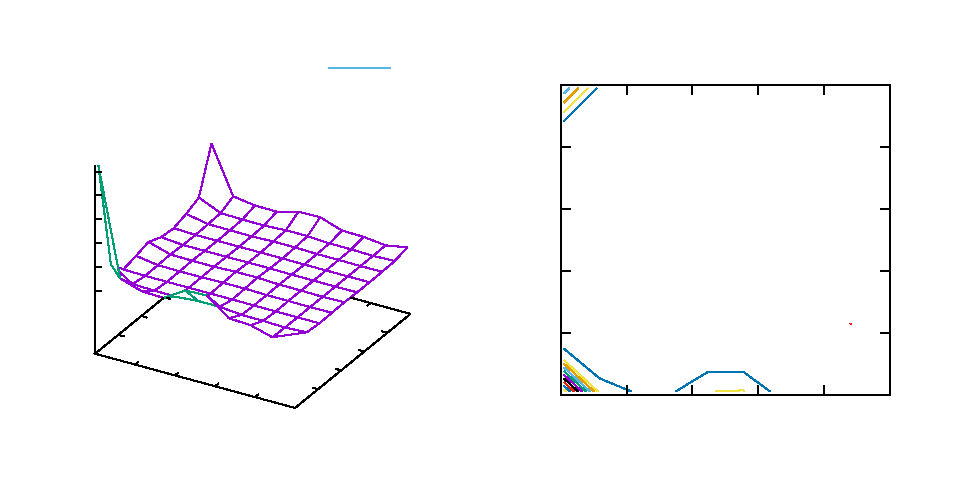
\includegraphics{plot_10_20_1000}}%
    \gplfronttext
  \end{picture}%
\endgroup
}
{\small Рис. 6 Плотность распределения указанной копулы}
\end{center}
\end{frame}

\begin{frame}
\begin{center}
\frametitle{Пример визуализации копулы для оценок границ компактов параметров $\sigma$ и $\lambda$ с б\'{о}льшим модельным значением}
\resizebox{\columnwidth}{!}{% GNUPLOT: LaTeX picture with Postscript
\begingroup
  \makeatletter
  \providecommand\color[2][]{%
    \GenericError{(gnuplot) \space\space\space\@spaces}{%
      Package color not loaded in conjunction with
      terminal option `colourtext'%
    }{See the gnuplot documentation for explanation.%
    }{Either use 'blacktext' in gnuplot or load the package
      color.sty in LaTeX.}%
    \renewcommand\color[2][]{}%
  }%
  \providecommand\includegraphics[2][]{%
    \GenericError{(gnuplot) \space\space\space\@spaces}{%
      Package graphicx or graphics not loaded%
    }{See the gnuplot documentation for explanation.%
    }{The gnuplot epslatex terminal needs graphicx.sty or graphics.sty.}%
    \renewcommand\includegraphics[2][]{}%
  }%
  \providecommand\rotatebox[2]{#2}%
  \@ifundefined{ifGPcolor}{%
    \newif\ifGPcolor
    \GPcolortrue
  }{}%
  \@ifundefined{ifGPblacktext}{%
    \newif\ifGPblacktext
    \GPblacktextfalse
  }{}%
  % define a \g@addto@macro without @ in the name:
  \let\gplgaddtomacro\g@addto@macro
  % define empty templates for all commands taking text:
  \gdef\gplbacktext{}%
  \gdef\gplfronttext{}%
  \makeatother
  \ifGPblacktext
    % no textcolor at all
    \def\colorrgb#1{}%
    \def\colorgray#1{}%
  \else
    % gray or color?
    \ifGPcolor
      \def\colorrgb#1{\color[rgb]{#1}}%
      \def\colorgray#1{\color[gray]{#1}}%
      \expandafter\def\csname LTw\endcsname{\color{white}}%
      \expandafter\def\csname LTb\endcsname{\color{black}}%
      \expandafter\def\csname LTa\endcsname{\color{black}}%
      \expandafter\def\csname LT0\endcsname{\color[rgb]{1,0,0}}%
      \expandafter\def\csname LT1\endcsname{\color[rgb]{0,1,0}}%
      \expandafter\def\csname LT2\endcsname{\color[rgb]{0,0,1}}%
      \expandafter\def\csname LT3\endcsname{\color[rgb]{1,0,1}}%
      \expandafter\def\csname LT4\endcsname{\color[rgb]{0,1,1}}%
      \expandafter\def\csname LT5\endcsname{\color[rgb]{1,1,0}}%
      \expandafter\def\csname LT6\endcsname{\color[rgb]{0,0,0}}%
      \expandafter\def\csname LT7\endcsname{\color[rgb]{1,0.3,0}}%
      \expandafter\def\csname LT8\endcsname{\color[rgb]{0.5,0.5,0.5}}%
    \else
      % gray
      \def\colorrgb#1{\color{black}}%
      \def\colorgray#1{\color[gray]{#1}}%
      \expandafter\def\csname LTw\endcsname{\color{white}}%
      \expandafter\def\csname LTb\endcsname{\color{black}}%
      \expandafter\def\csname LTa\endcsname{\color{black}}%
      \expandafter\def\csname LT0\endcsname{\color{black}}%
      \expandafter\def\csname LT1\endcsname{\color{black}}%
      \expandafter\def\csname LT2\endcsname{\color{black}}%
      \expandafter\def\csname LT3\endcsname{\color{black}}%
      \expandafter\def\csname LT4\endcsname{\color{black}}%
      \expandafter\def\csname LT5\endcsname{\color{black}}%
      \expandafter\def\csname LT6\endcsname{\color{black}}%
      \expandafter\def\csname LT7\endcsname{\color{black}}%
      \expandafter\def\csname LT8\endcsname{\color{black}}%
    \fi
  \fi
    \setlength{\unitlength}{0.0500bp}%
    \ifx\gptboxheight\undefined%
      \newlength{\gptboxheight}%
      \newlength{\gptboxwidth}%
      \newsavebox{\gptboxtext}%
    \fi%
    \setlength{\fboxrule}{0.5pt}%
    \setlength{\fboxsep}{1pt}%
\begin{picture}(9070.00,4534.00)%
    \gplgaddtomacro\gplbacktext{%
    }%
    \gplgaddtomacro\gplfronttext{%
      \csname LTb\endcsname%
      \put(2863,4030){\makebox(0,0)[r]{\strut{}$\widehat{p}_\sigma=0.707107$, $\widehat{p}_{x_m}=0.125$}}%
      \csname LTb\endcsname%
      \put(683,1188){\makebox(0,0){\strut{}\ft $0$}}%
      \put(1067,1084){\makebox(0,0){\strut{}\ft $0.2$}}%
      \put(1451,979){\makebox(0,0){\strut{}\ft $0.4$}}%
      \put(1835,875){\makebox(0,0){\strut{}\ft $0.6$}}%
      \put(2219,771){\makebox(0,0){\strut{}\ft $0.8$}}%
      \put(2602,667){\makebox(0,0){\strut{}\ft $1$}}%
      \put(1436,797){\makebox(0,0){\strut{}$\widehat{p}_\sigma$}}%
      \put(2787,710){\makebox(0,0){\strut{}\ft $0$}}%
      \put(3008,891){\makebox(0,0){\strut{}\ft $0.2$}}%
      \put(3230,1071){\makebox(0,0){\strut{}\ft $0.4$}}%
      \put(3452,1252){\makebox(0,0){\strut{}\ft $0.6$}}%
      \put(3673,1433){\makebox(0,0){\strut{}\ft $0.8$}}%
      \put(3895,1613){\makebox(0,0){\strut{}\ft $1$}}%
      \put(3706,1083){\makebox(0,0){\strut{}$\widehat{p}_{x_m}$}}%
      \put(627,1886){\makebox(0,0)[r]{\strut{}\ft $0$}}%
      \put(627,1920){\makebox(0,0)[r]{\strut{}\ft $3$}}%
      \put(627,1955){\makebox(0,0)[r]{\strut{}\ft $6$}}%
      \put(627,1990){\makebox(0,0)[r]{\strut{}\ft $9$}}%
      \put(627,2024){\makebox(0,0)[r]{\strut{}\ft $12$}}%
      \put(627,2059){\makebox(0,0)[r]{\strut{}\ft $15$}}%
      \put(627,2094){\makebox(0,0)[r]{\strut{}\ft $18$}}%
      \put(627,2129){\makebox(0,0)[r]{\strut{}\ft $21$}}%
      \put(627,2163){\makebox(0,0)[r]{\strut{}\ft $24$}}%
      \put(627,2198){\makebox(0,0)[r]{\strut{}\ft $27$}}%
      \put(627,2233){\makebox(0,0)[r]{\strut{}\ft $30$}}%
      \put(627,2267){\makebox(0,0)[r]{\strut{}\ft $33$}}%
      \put(627,2302){\makebox(0,0)[r]{\strut{}\ft $36$}}%
      \put(627,2337){\makebox(0,0)[r]{\strut{}\ft $39$}}%
      \put(627,2372){\makebox(0,0)[r]{\strut{}\ft $42$}}%
      \put(627,2405){\makebox(0,0)[r]{\strut{}\ft $45$}}%
      \put(627,2440){\makebox(0,0)[r]{\strut{}\ft $48$}}%
      \put(627,2475){\makebox(0,0)[r]{\strut{}\ft $51$}}%
      \put(627,2510){\makebox(0,0)[r]{\strut{}\ft $54$}}%
      \put(627,2544){\makebox(0,0)[r]{\strut{}\ft $57$}}%
      \put(627,2579){\makebox(0,0)[r]{\strut{}\ft $60$}}%
      \put(627,2614){\makebox(0,0)[r]{\strut{}\ft $63$}}%
      \put(627,2648){\makebox(0,0)[r]{\strut{}\ft $66$}}%
      \put(627,2683){\makebox(0,0)[r]{\strut{}\ft $69$}}%
      \put(627,2718){\makebox(0,0)[r]{\strut{}\ft $72$}}%
      \put(627,2753){\makebox(0,0)[r]{\strut{}\ft $75$}}%
      \put(627,2787){\makebox(0,0)[r]{\strut{}\ft $78$}}%
      \put(627,2822){\makebox(0,0)[r]{\strut{}\ft $81$}}%
      \put(627,2857){\makebox(0,0)[r]{\strut{}\ft $84$}}%
      \put(627,2891){\makebox(0,0)[r]{\strut{}\ft $87$}}%
      \put(627,2926){\makebox(0,0)[r]{\strut{}\ft $90$}}%
      \put(627,2961){\makebox(0,0)[r]{\strut{}\ft $93$}}%
      \put(627,2996){\makebox(0,0)[r]{\strut{}\ft $96$}}%
      \put(627,3030){\makebox(0,0)[r]{\strut{}\ft $99$}}%
      \put(627,3065){\makebox(0,0)[r]{\strut{}\ft $102$}}%
      \put(-171,2487){\makebox(0,0){\strut{}$\widehat{c}$}}%
    }%
    \gplgaddtomacro\gplbacktext{%
    }%
    \gplgaddtomacro\gplfronttext{%
      \csname LTb\endcsname%
      \put(5223,578){\makebox(0,0){\strut{}\ft $0$}}%
      \put(5855,578){\makebox(0,0){\strut{}\ft $0.2$}}%
      \put(6487,578){\makebox(0,0){\strut{}\ft $0.4$}}%
      \put(7117,578){\makebox(0,0){\strut{}\ft $0.6$}}%
      \put(7749,578){\makebox(0,0){\strut{}\ft $0.8$}}%
      \put(8381,578){\makebox(0,0){\strut{}\ft $1$}}%
      \put(6802,248){\makebox(0,0){\strut{}$\widehat{p}_\sigma$}}%
      \put(5035,891){\makebox(0,0)[r]{\strut{}\ft $0$}}%
      \put(5035,1486){\makebox(0,0)[r]{\strut{}\ft $0.2$}}%
      \put(5035,2080){\makebox(0,0)[r]{\strut{}\ft $0.4$}}%
      \put(5035,2674){\makebox(0,0)[r]{\strut{}\ft $0.6$}}%
      \put(5035,3268){\makebox(0,0)[r]{\strut{}\ft $0.8$}}%
      \put(5035,3863){\makebox(0,0)[r]{\strut{}\ft $1$}}%
      \put(4309,2377){\rotatebox{-270}{\makebox(0,0){\strut{}$\widehat{p}_{x_m}$}}}%
    }%
    \gplbacktext
    \put(0,0){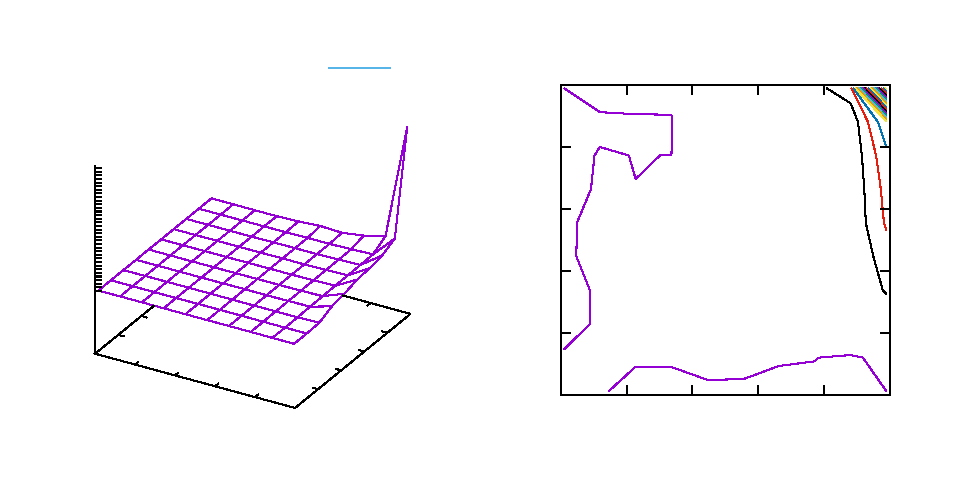
\includegraphics{images/plots/plot_10_21_1000}}%
    \gplfronttext
  \end{picture}%
\endgroup
}
{\small Рис. 7 Плотность распределения указанной копулы}
\end{center}
\end{frame}

\setbeamertemplate{frametitle}
{
  \nointerlineskip
  \begin{beamercolorbox}[wd=\paperwidth,leftskip=0.3cm,rightskip=0.3cm,ht=2.5ex,dp=1.5ex]{frametitle}
    \usebeamerfont{frametitle}%
    \scshape \protect\insertframetitle%
  \end{beamercolorbox}%

  \if@useTitleProgressBar
    \nointerlineskip
    \begin{beamercolorbox}[wd=\paperwidth,ht=0.4pt,dp=0pt]{frametitle}
      \progressbar{\paperwidth}
    \end{beamercolorbox}
  \fi
}
\makeatother

\begin{frame}
\begin{center}
\frametitle{Один из выводов на основе результатов оценивания}
\begin{itemize}
  \item Оценка в форме копулы подтвердила априорные предположения о характере связи результатов построения компактов для $\sigma$ и $x_m$;
  \item При малом модельном значении $x_m$ оценка копулы позволяет выделить подмножество пар значений параметров, для которых необходимо провести следующий этап исследований свойств композиции алгоритмов построения интервальных оценок;
\end{itemize}
\end{center}
\end{frame}

\begin{frame}
\begin{center}
\frametitle{Результаты}
\begin{itemize}
  \item Создан программный пакет, позволяющий строить вероятностные модели в форме композиции распределений и копул;
  \item Построены оценки копул согласно модели процесса \eqref{eq:x} (243 шт.);
  \item Эти оценки выявили ряд зависимостей между результатами построения границ компактов в параметрическом пространстве процесса \eqref{eq:x};
  \item Такие зависимости --- основание для проведения дальнейших исследований алгоритма построения границ компакта, причём копула обеспечивает нас информацией о том, на каком подмножестве пар значений параметров следует сосредоточить внимание;
\end{itemize}
\end{center}
\end{frame}

\begin{frame}
\begin{center}
\frametitle{Результаты $(1)$}
\begin{itemize}
  \item Описанный подход может быть применён для анализа результатов оценивания параметров моделей произвольных случайных процессов;
  \item Реализованное ПО можно использовать для решения широкого круга задач из класса Data Mining;
\end{itemize}
\end{center}
\end{frame}

\begin{frame}
\begin{center}
Спасибо за внимание!
\end{center}
\end{frame}

\begin{frame}
\frametitle{Пуассоновский поток событий $Y(t)$}
\[Y(t) = \sum_{j = 0}^K P_j \cdot I(t - \tau_j) \cdot e^{-\lambda_c(t - \tau_j)}\]
Интервал времени между моментами возникновения возмущений --- случайная величина, распределённая по экспоненциальному закону с параметром $\lambda$:
\begin{gather}
\Delta \tau_j = t_j - t_{j-1} \\
\Delta \tau_j \sim Exp(\lambda).
\end{gather}
\end{frame}

\begin{frame}
\frametitle{Копулы}
\emph{Двумерной копулой} называется функция $C$, удовлетворяющая следующим свойствам:
\begin{enumerate}
\item $\Dom{C} = I^2$;
\item $\forall u,v \in I : C(u, 0) = 0 = C(0, v)$;
\item $\forall B = [x_1, x_2] \times [y_1, y_2] \subset I^2 : \Diff_{y_1}^{y_2}\Diff_{x_1}^{x_2}C(x, y) \geqslant 0$;
\item Для каждых $u, v \in I$:
  \begin{gather}
    C(u, 1) = u \\
    C(1, v) = v.
  \end{gather}
\end{enumerate}
\end{frame}

\begin{frame}
\frametitle{Примеры копул}
\begin{figure}[H]
  \centering
  \begin{subfigure}{.3\textwidth}
    \centering
    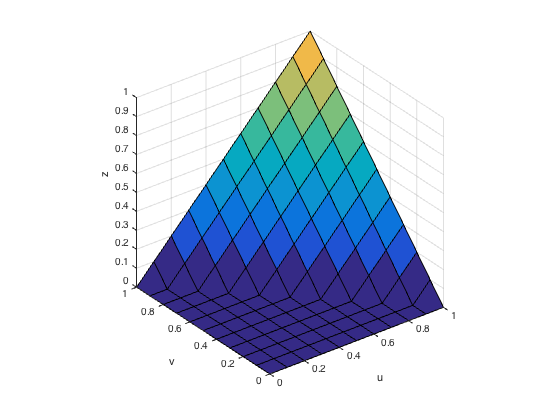
\includegraphics[width=\linewidth]{W.png}
    \caption{$z = W(u, v)$}
  \end{subfigure}%
  \begin{subfigure}{.3\textwidth}
    \centering
    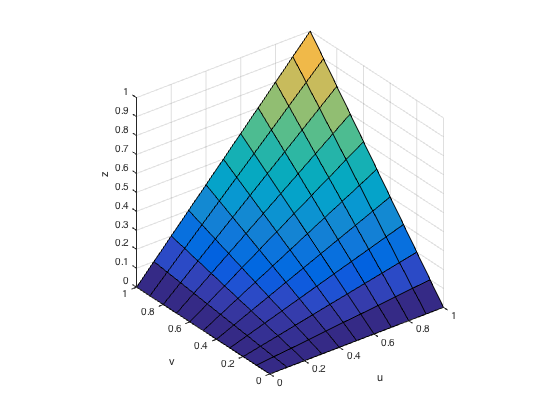
\includegraphics[width=\linewidth]{P.png}
    \caption{$z = P(u, v)$}
  \end{subfigure}
  \begin{subfigure}{.3\textwidth}
    \centering
    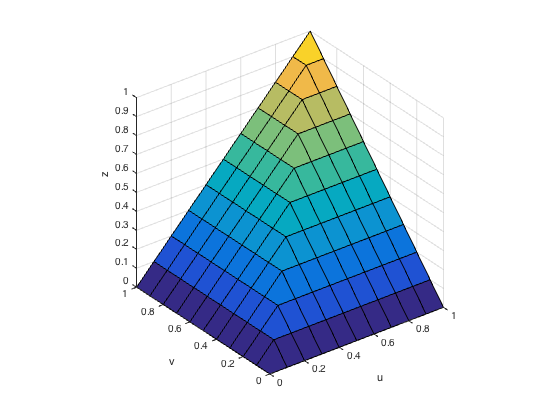
\includegraphics[width=\linewidth]{M.png}
    \caption{$z = M(u, v)$}
  \end{subfigure}
  \caption{Графики копул $W$, $P$ и $M$}
\end{figure}
\end{frame}

\begin{frame}
\frametitle{Теорема Скляра и теорема об инвариантности}
\begin{itemize}
\item Пусть $X, Y$ --- случайные величины с распределениями $F, G$ соответственно, и совместным распределением $H$. Тогда выполняется уравнение
\begin{equation}
  H(x, y) = C(F(x), G(y)).
\end{equation}
Если $F$ и $G$ непрерывны, то $C$ единственна;

\item Пусть $X, Y$ --- непрерывные случайные величины c копулой $C_{XY}$. Если $\alpha$ и $\beta$ строго возрастают на $\Ran{X}$ и $\Ran{Y}$ соответственно, то $C_{\alpha(X)\beta(Y)} = C_{XY}$. Таким образом $C_{XY}$ инвариантна относительно строго возрастающих преобразований $X$ и $Y$.
\end{itemize}
\end{frame}

\begin{frame}
\frametitle{Коэффициент корреляции Пирсона}
\begin{figure}\label{fig:pearson}
\centering
\begin{subfigure}{.45\textwidth}
  \centering
  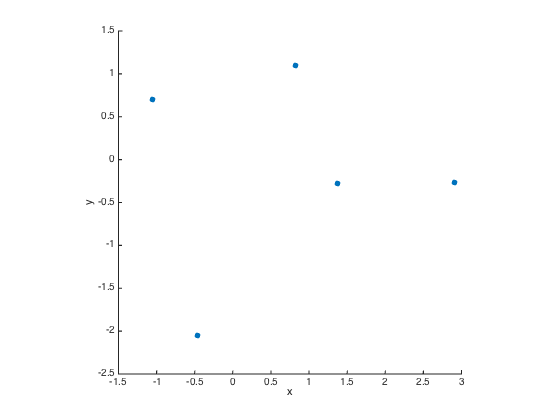
\includegraphics[width = \textwidth]{./images/normscatter.png}
  \caption{$(x, y) \sim \mathcal{N}, \rho = 0.06 $}
  \label{fig:norm}
\end{subfigure}
\begin{subfigure}{.45\textwidth}
  \centering
  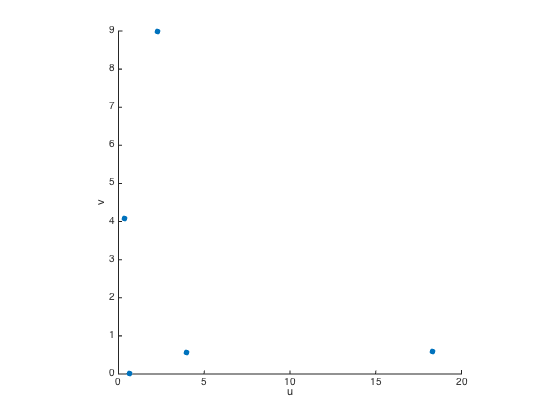
\includegraphics[width = \textwidth]{./images/transformed_normscatter.png}
  \caption{$(x, y) = (\e^x, \e^{2y}), \rho = -0.33$}
  \label{fig:transnorm}
\end{subfigure}
\end{figure}
\end{frame}

\begin{frame}
\frametitle{Коэффициент ранговой корреляции Кендалла}
\begin{itemize}
  \item \emph{Коэффициентом ранговой корреляции} вектора случайных величин $\trans{(X, Y)}$ называется величина
\begin{equation}
  \tau(X, Y) = \P\{\, (X - \widetilde{X})(Y - \widetilde{Y}) > 0 \,\} - \P\{\, (X - \widetilde{X})(Y - \widetilde{Y}) < 0 \,\},
\end{equation}
где $\trans{(\widetilde{X}, \widetilde{Y})}$ --- независимая копия $\trans{(X, Y)}$. \par

\item Пусть $X, Y$ --- непрерывные случайные величины с копулой $C$, тогда их коэффициенту Кендалла соответствует выражение
  \[
  \tau(X, Y) = \tau_C = 4 \iint_{I^2} C(u, v) \d C(u,v) - 1.
  \]
\end{itemize}
\end{frame}

\end{document}
